\documentclass{article}
\usepackage{amsmath, amssymb, bm}
\usepackage{braket}

% Enhanced packages for better document structure
\usepackage{titlesec}
\usepackage{tocloft}
\usepackage{amsthm}
\usepackage{thmtools}
\usepackage{mdframed}
\usepackage{enumitem}
\usepackage{geometry}
\usepackage{xcolor}
\usepackage{tikz} % Added for circuit diagrams

% Set better margins
\geometry{margin=1in}

% Configure theorem-like environments
\newtheorem{theorem}{Theorem}[subsection]
\newtheorem{definition}[theorem]{Definition}
\newtheorem{example}[theorem]{Example}

% Define a nice box for important concepts
\newmdenv[
  linewidth=0.5pt,
  skipabove=1em,
  skipbelow=1em,
  backgroundcolor=gray!10,
  innerleftmargin=5pt,
  innerrightmargin=5pt,
  innertopmargin=5pt,
  innerbottommargin=5pt
]{conceptbox}

% Configure section formatting for chapters
\titleformat{\section}
  {\LARGE\bfseries}{\thesection.}{1em}{\MakeUppercase}
\titlespacing*{\section}{0pt}{3.5ex plus 1ex minus .2ex}{2.3ex plus .2ex}

% Configure subsection and subsubsection formatting
\titleformat{\subsection}
  {\Large\bfseries}{\thesubsection}{1em}{}
\titleformat{\subsubsection}
  {\large\bfseries}{\thesubsubsection}{1em}{}

% Configure spacing
\titlespacing*{\subsection}{0pt}{3.25ex plus 1ex minus .2ex}{1.5ex plus .2ex}
\titlespacing*{\subsubsection}{0pt}{3.25ex plus 1ex minus .2ex}{1.5ex plus .2ex}

% Configure list spacing
\setlist{itemsep=0.5em}

% Configure TOC depth and formatting
\setcounter{tocdepth}{3}
\renewcommand{\cftsecfont}{\Large\bfseries}
\renewcommand{\cftsecpagefont}{\bfseries}
\renewcommand{\cftsubsecindent}{2em}
\renewcommand{\cftsubsubsecindent}{4em}

\title{Advanced Electromagnetism I}
\author{PHYS 435}
\date{Fall 2025}

\begin{document}
\maketitle

\newpage
\tableofcontents

%%%%%%%%%%%%%%%%%%%%%%%%%%%%%%%%%%%%%%%%%%%%%%%% New Chapter %%%%%%%%%%%%%%%%%%%%%%%%%%%%%%%%%%%%%%%%%%%%%%%%
\newpage
\section{Lecture 2: Gauss's Law}
\subsubsection*{August 27, 2025}

\subsection{Gauss's Law}
\begin{conceptbox}
The electric field from a collection of charges is the vector sum of the fields from each charge.
\begin{align*}
    \vec{E} = \frac{1}{4\pi\epsilon_0}\sum_{i=1}^N \frac{q_i}{|\vec{r}_i|^2} \hat{\vec{r}}_i,\text{ } \vec{r}_i=\vec{r}-\vec{r'}_i
\end{align*}
\end{conceptbox}

\subsection{Gauss's Law in Differential Form}
\begin{conceptbox}
The divergence of the electric field is proportional to the charge density.
\begin{align*}
    \oint_C v(\vec{r}) \cdot d\vec{a} = \int_v (\mathcal{r}\cdot\vec{v}(\vec{r}))d\tau \\
    \vec{v}(\vec{r}) = \text{any differentiable vector field} \\
    \mathcal{r}\cdot\vec{v} = \text{divergence} = \frac{\partial v_x}{\partial x} + \frac{\partial v_y}{\partial y} + \frac{\partial v_z}{\partial z} \\
    \text{Apply to Gauss's Law}: \\
    \oint \vec{E} \cdot d\vec{a} = \int_v (\mathcal{r}\cdot\vec{E}(\vec{r}))d\tau = \frac{Q_{enc}}{\epsilon_0}, \text{ } Q_{enc} = \int_v \rho(\vec{r})d\tau \\
    \int_v(\mathcal{r}\cdot\vec{E})d\tau = \int_v(\rho(\vec{r})/\epsilon_0)d\tau \\
    \nabla\cdot\vec{E}(\vec{r}) = \frac{\rho(\vec{r})}{\epsilon_0} \\
    \text{Divergence Identity: }\\
    \mathcal{r}_r\cdot(\frac{\vec{r}}{r^2}) = 4\pi\delta^3(\vec{r}) \\
\end{align*}
\end{conceptbox}

\section{Lecture 3: The curl of $\vec{E}(\nabla\times\vec{E})$}
\subsubsection*{August 29, 2025}
\begin{conceptbox}
Integral:
\begin{align*}
    \oint_C \vec{E} \cdot d\vec{a} = \frac{Q_{enc}}{\epsilon_0}
\end{align*}
Differential:
\begin{align*}
    \nabla\times\vec{E}(\vec{r}) = \frac{\rho(\vec{r})}{\epsilon_0}
\end{align*}
\end{conceptbox}

\subsection{Problem 2.18 Griffiths}
Approach: Use superposition to add contributions from each sphere.

\subsection{Practice using the differential form of Gauss's Law}
\begin{example}
    For the differential form, it is important to remember we are considering a specified point in space.
\begin{align*}
    \text{Consider two identical charged plates and the electric field between them is constant.} \\
    \text{The charge density is $0$ between the plates.} \nabla\cdot\vec{E}=0, \nabla\cdot\vec{E}=\frac{\rho}{\epsilon_0} \Rightarrow \text{Charge density is 0} \\
    \nabla\cdot\vec{E}\neq0 \Rightarrow \text{charge density}
\end{align*}
\end{example}

\begin{example}
    Now consider $\nabla\times\vec{E}$ (curl)
    \begin{align*}
        \text{By Stokes's theorem: } \int_S (\nabla \times \vec{v}) \cdot d\vec{a} = \oint_C \vec{v} \cdot d\vec{l}
    \end{align*}
\end{example}
\begin{conceptbox}
The curl of any electric field due to a fixed charge distribution is zero:
\[
\nabla \times \vec{E}(\vec{r}) = 0
\]
For any closed loop,
\[
\oint \vec{E} \cdot d\vec{l} = 0
\]
\end{conceptbox}


%%%%%%%%%%%%%%%%%%%%%%%%%%%%%%%%%%%%%%%%%%%%%%%% New Chapter %%%%%%%%%%%%%%%%%%%%%%%%%%%%%%%%%%%%%%%%%%%%%%%%
\newpage
\section{Lecture 4: Electric Potential}
\subsubsection*{September 3, 2025}

\subsection{Electric Potential}
For static charge distributions
\begin{align*}
    \mathcal{r}\times\vec{E} = 0 \rightarrow \text{implies that 3 components of $\vec{E}$ are related to each other.}
\end{align*}
Stokes's Theorem states that:
\begin{center}
\begin{align*}
    &\int_S (\mathcal{r} \times \vec{E}) \cdot d\vec{a} = \oint_P \vec{E} \cdot d\vec{l} \\[1.5ex]
    &\oint_P \vec{E} \cdot d\vec{l} = 0 \\[1.5ex]
    &\oint_P \vec{E} \cdot d\vec{l} \text{ is independent of path} \\[1.5ex]
    &\int_a^b \vec{E} \cdot d\vec{l} + \int_b^a \vec{E} \cdot d\vec{l} = 0 \\[1.5ex]
    &\text{Only the endpoints $a$ and $b$ matter} \\[1.5ex]
    &\text{We can define a scalar function $V(\vec{r})$ such that:} \\[0.5ex]
    &\int_a^b \vec{E} \cdot d\vec{l} = V(\vec{a}) - V(\vec{b}) \\
    &V(\vec{r}) = - \int_a^r \vec{E} \cdot d\vec{l} \\
    &V(b)-V(a)=-\int_0^b \vec{E} \cdot d\vec{l}+\int_0^a \vec{E} \cdot d\vec{l}=-\int_a^b \vec{E} \cdot d\vec{l} \\
    &\text{Fundamental thereom of gradients: } V(b)-V(a)=\int_a^b\nabla V\cdot d\vec{l} \\
    &\rightarrow \vec{E}=-\nabla V(\vec{r})
\end{align*}
\end{center}

\subsection{Potential}
\begin{center}
\begin{align*}
    &\text{1. $V$ is the (electric) potential.} \\
    &E = \frac{N}{C}, \quad V = \frac{N \cdot m}{C} = \frac{J}{C} = \text{Volt} \\
    &\text{2. The potential at one point has no physical significance.} \\
    &\text{Potential differences matter. We always define some reference point $O$.} \\
    &\text{Typically choose $O$ such that $V(O)=0$. We can always change the} \\
    &\text{reference point if we wish $V(\vec{r})\rightarrow V(\vec{r})+C$.} \\
    &\vec{E}\rightarrow\vec{E} \\
    &\text{3. Superposition also works with the potential} \\
    &\vec{E}=\vec{E}_1+\vec{E}_2+\cdots+\vec{E}_N \\
    &\vec{E}=-\nabla V \text{ or } V(\vec{r})=-\int_0^r \vec{E} \cdot d\vec{l} \\
    &V_{total}=-\int_0^r \vec{E}_1 \cdot d\vec{l} + -\int_0^r \vec{E}_2 \cdot d\vec{l} + \cdots + -\int_0^r \vec{E}_N \cdot d\vec{l} \\
    &= v_1(\vec{r}) + v_2(\vec{r}) + \cdots + v_N(\vec{r}) \\
\end{align*}
\end{center}
\example[Potential due to a point charge]

\begin{center}
\begin{minipage}{0.45\textwidth}
    \begin{center}
    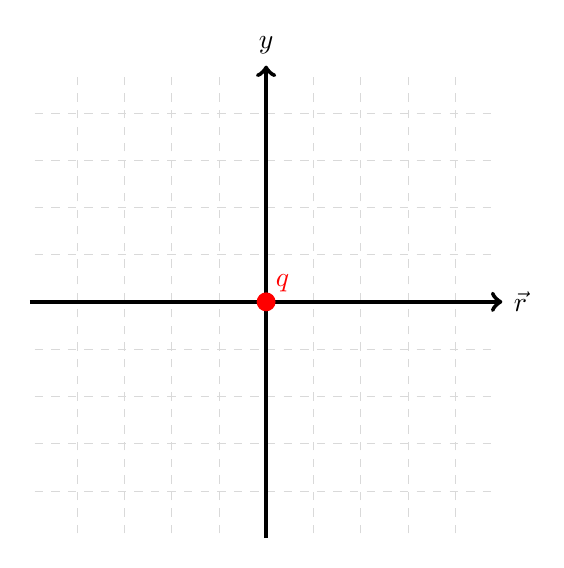
\begin{tikzpicture}[scale=0.6]
        \draw[help lines, color=gray!30, dashed] (-4.9,-4.9) grid (4.9,4.9);
        \draw[->,ultra thick] (-5,0)--(5,0) node[right]{$\vec{r}$};
        \draw[->,ultra thick] (0,-5)--(0,5) node[above]{$y$};
        \fill[red] (0,0) circle (0.2) node[above right]{$q$};
    \end{tikzpicture}
    \end{center}
\end{minipage}
\hfill
\begin{minipage}{0.45\textwidth}
    \begin{align*}
        &\vec{E}=\frac{q}{4\pi\epsilon_0}\frac{1}{r^2}\vec{r} \\
        &V(\vec{r})=-\int_0^{\vec{r}} \vec{E} \cdot d\vec{l} \\
        &=-\int_{\infty}^r \frac{q}{4\pi\epsilon_0}\frac{1}{r'^2} dr' \\
        &=\frac{q}{4\pi\epsilon_0}\frac{1}{r}
    \end{align*}
\end{minipage}
\end{center}

\subsection{Poisson's Equation}
\begin{align*}
    \vec{E}=-\nabla V, \text{Gauss's law} \nabla\cdot\vec{E}(\vec{r})=\frac{\rho(\vec{r})}{\epsilon_0} \rightarrow \nabla^2 V = \frac{\rho(\vec{r})}{\epsilon_0} + \text{Boundary conditions}
\end{align*}


%%%%%%%%%%%%%%%%%%%%%%%%%%%%%%%%%%%%%%%%%%%%%%%% New Chapter %%%%%%%%%%%%%%%%%%%%%%%%%%%%%%%%%%%%%%%%%%%%%%%%
\newpage
\section{Lecture 5: Electrostatic Boundary Conditions}
\subsubsection*{September 5, 2025 \\}

Recall: $\vec{E}(\vec{r}) = -\nabla V(\vec{r})$, and also $\nabla^2 V(\vec{r}) = \frac{\rho(\vec{r})}{\epsilon_0}$. \\

Invert: $\nabla^2 V(\vec{r}) = -\frac{\rho(\vec{r})}{\epsilon_0} \rightarrow V(\vec{r}) = f(p)$. \\

For a point charge, $V(\vec{r}) = \frac{q}{4\pi\epsilon_0 \mathcal{r}}$, where $\vec{\mathcal{r}} = \vec{r} - \vec{r}'$. \\

If we add another charge, $V(\vec{r}) = \frac{q}{4\pi\epsilon_0 \mathcal{r}} + \frac{q'}{4\pi\epsilon_0 \mathcal{r}'}$ (just superpose). \\

For $N$ charges: $V(\vec{r}) = \sum_{i=1}^N \frac{q_i}{4\pi\epsilon_0 \mathcal{r}_i}$. \\

For a continuous distribution: $V(\vec{r}) = \int \frac{dq}{4\pi\epsilon_0 \mathcal{r}} = \int \frac{\rho(\vec{r}')}{4\pi\epsilon_0 \mathcal{r}} d\tau'$. \\

For a line charge: $V(\vec{r}) = \int \frac{\lambda(\vec{r}')}{4\pi\epsilon_0 \mathcal{r}} dl'$. \\

For a surface charge: $V(\vec{r}) = \int \frac{\sigma(\vec{r}')}{4\pi\epsilon_0 \mathcal{r}} da'$. \\

For a volume charge: $V(\vec{r}) = \int \frac{\rho(\vec{r}')}{4\pi\epsilon_0 \mathcal{r}} d\tau'$.

\newpage
\subsection{Line Charge}
\example[Find e-field from line charge]

\begin{center}
\begin{minipage}{0.48\textwidth}
    \centering
    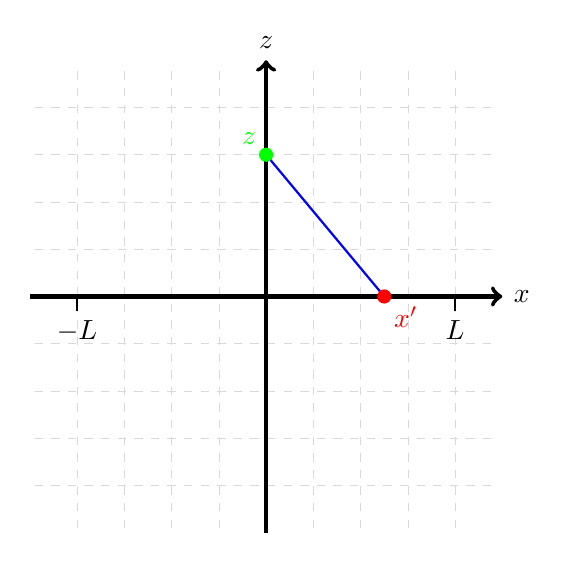
\begin{tikzpicture}[scale=0.6]
        \draw[help lines, color=gray!30, dashed] (-4.9,-4.9) grid (4.9,4.9);
        \draw[->,ultra thick] (-5,0)--(5,0) node[right]{$x$};
        \draw[->,ultra thick] (0,-5)--(0,5) node[above]{$z$};
        \draw[thick] (-4,0) -- (-4,-0.3) node[below]{$-L$};
        \draw[thick] (4,0) -- (4,-0.3) node[below]{$L$};
        \coordinate (xprime) at (2.5,0);
        \coordinate (zpoint) at (0,3);
        \draw[thick, blue] (xprime) -- (zpoint);
        \fill[red] (xprime) circle (0.15) node[below right]{$x'$};
        \fill[green] (zpoint) circle (0.15) node[above left]{$z$};
    \end{tikzpicture}
\end{minipage}%
\hfill
\begin{minipage}{0.48\textwidth}
    \vspace{0.5em}
    \begin{align*}
        &\int dV = \int \frac{dq}{4\pi\epsilon_0\mathcal{r}} = \int \frac{\lambda dx'}{4\pi\epsilon_0\sqrt{x'^2+z^2}} \\
        &V = \frac{\lambda}{4\pi\epsilon_0} \int_{-L}^L \frac{dx'}{\sqrt{x'^2+z^2}} = \frac{\lambda}{4\pi\epsilon_0} \left[\ln(x'+\sqrt{x'^2+z^2})\right]_{-L}^L \\
        &V(z) = \frac{\lambda}{4\pi\epsilon_0} \ln\left(\frac{L+\sqrt{L^2+z^2}}{-L+\sqrt{L^2+z^2}}\right) \\
        &\vec{E}=-\nabla V = -(\frac{\partial V}{\partial x}\hat{x}+\frac{\partial V}{\partial y}\hat{y}+\frac{\partial V}{\partial z}\hat{z}) = -\frac{\partial V}{\partial z}\hat{z} = \frac{2L\lambda}{4\pi\epsilon_0} \frac{1}{z\sqrt{L^2+z^2}} \hat{z} \\
    \end{align*}
\end{minipage}
\end{center}

\newpage
\subsection{Spherical Shell}

\begin{example}[Spherical Shell]
\begin{center}
\begin{minipage}{0.48\textwidth}
    \centering
    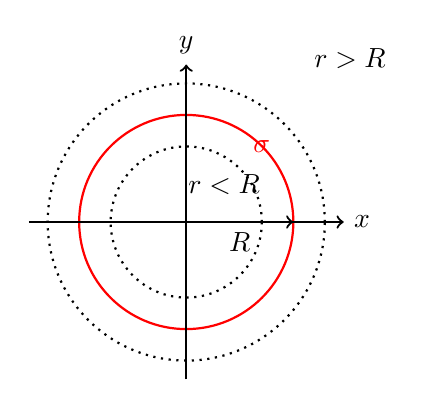
\begin{tikzpicture}[scale=0.8]
        % Draw dotted circles smaller and larger than the shell
        \draw[dotted, thick] (0,0) circle (1.2);
        \draw[dotted, thick] (0,0) circle (2.2);
        
        % Draw the main spherical shell with radius R
        \draw[thick, red] (0,0) circle (1.7);
        
        % Add surface charge density label
        \node[red] at (1.2, 1.2) {$\sigma$};
        
        % Add radius label
        \draw[thick, ->] (0,0) -- (1.7,0) node[midway, below]{$R$};
        
        % Add labels for the dotted circles
        \node at (0.6, 0.6) {$r < R$};
        \node at (2.6, 2.6) {$r > R$};
        
        % Add coordinate axes
        \draw[->, thick] (-2.5,0) -- (2.5,0) node[right]{$x$};
        \draw[->, thick] (0,-2.5) -- (0,2.5) node[above]{$y$};
    \end{tikzpicture}
\end{minipage}%
\hfill
\begin{minipage}{0.48\textwidth}
    \vspace{0.5em}
    \begin{align*}
        &\text{Spherical shell with radius } R \text{ and surface charge density } \sigma \\
        &\text{For } r < R: \quad Q_{enc}=0, \quad \vec{E} = 0 \\
        &\text{For } r > R: \quad \oint\vec{E}\cdot d\vec{a}=\frac{Q_{enc}}{\epsilon_0}, \quad \vec{E} = \frac{\sigma}{\epsilon_0}\frac{R^2}{r^2} \hat{r} \quad \text{where } Q_{enc} = 4\pi R^2 \sigma\\
        &\text{At } r = R: \quad E_{\text{out}} - E_{\text{in}} = \frac{\sigma}{\epsilon_0} \\
        &\text{Since } E_{\text{in}} = 0: \quad E_{\text{out}} = \frac{\sigma}{\epsilon_0}
    \end{align*}
\end{minipage}
\end{center}

\vspace{1em}

\begin{center}
\begin{tikzpicture}[scale=1.1]
    % Axes
    \draw[->, thick] (0,0) -- (5.2,0) node[right] {$r$};
    \draw[->, thick] (0,0) -- (0,3.2) node[above] {$E$};

    % E field: E=0 for r<R, jump at R, then decays as 1/r^2
    \draw[thick, blue] (0,0) -- (2,0); % E=0 for r<R

    % Vertical jump at r=R
    \draw[dashed] (2,0) -- (2,2.5);
    \filldraw[black] (2,2.5) circle (1.2pt);

    % Label R on x-axis
    \draw (2,-0.15) -- (2,0.15);
    \node[below] at (2,0) {$R$};

    % Label delta E at (R, E)
    \node[right] at (2.05,2.5) {$\Delta E = \frac{\sigma}{\epsilon_0}$};

    % E for r>R: decays as 1/r^2, but for sketch, just a curve
    \draw[thick, blue, domain=2:5, samples=100] plot (\x,{2.5*4/(\x*\x)});

    % Dotted line at E = sigma/epsilon_0
    \draw[dotted] (0,2.5) -- (2,2.5);

    % Label E axis at delta E
    \node[left] at (0,2.5) {$\frac{\sigma}{\epsilon_0}$};
\end{tikzpicture}
\end{center}
\end{example}

\newpage
\subsection{Sheet of Charge}
\begin{example}[Imagine sheet of charge]
\begin{center}
\begin{minipage}{0.48\textwidth}
    \centering
    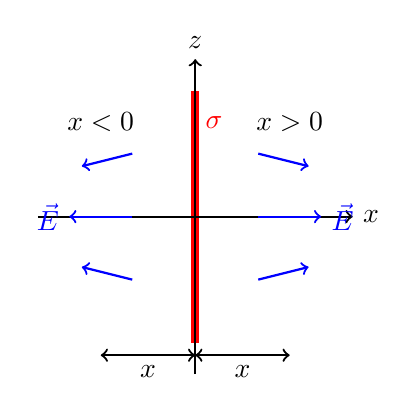
\begin{tikzpicture}[scale=0.8]
        % Draw the sheet of charge (vertical line)
        \draw[thick, red, line width=3pt] (0,-2) -- (0,2);
        
        % Add surface charge density label
        \node[red] at (0.3, 1.5) {$\sigma$};
        
        % Draw coordinate axes
        \draw[->, thick] (-2.5,0) -- (2.5,0) node[right]{$x$};
        \draw[->, thick] (0,-2.5) -- (0,2.5) node[above]{$z$};
        
        % Draw electric field lines
        \draw[->, thick, blue] (1,0) -- (2,0) node[right]{$\vec{E}$};
        \draw[->, thick, blue] (-1,0) -- (-2,0) node[left]{$\vec{E}$};
        \draw[->, thick, blue] (1,1) -- (1.8,0.8);
        \draw[->, thick, blue] (-1,1) -- (-1.8,0.8);
        \draw[->, thick, blue] (1,-1) -- (1.8,-0.8);
        \draw[->, thick, blue] (-1,-1) -- (-1.8,-0.8);
        
        % Add labels for regions
        \node at (1.5, 1.5) {$x > 0$};
        \node at (-1.5, 1.5) {$x < 0$};
        
        % Add distance labels
        \draw[<->, thick] (0,-2.2) -- (1.5,-2.2) node[midway, below]{$x$};
        \draw[<->, thick] (0,-2.2) -- (-1.5,-2.2) node[midway, below]{$x$};
    \end{tikzpicture}
\end{minipage}%
\hfill
\begin{minipage}{0.48\textwidth}
    \vspace{0.5em}
    \begin{align*}
        &\text{Infinite sheet of charge with surface density } \sigma \\
        &\text{Using Gauss's law with cylindrical Gaussian surface:} \\
        &\oint \vec{E} \cdot d\vec{a} = \frac{Q_{enc}}{\epsilon_0} \\
        &E \cdot 2A = \frac{\sigma A}{\epsilon_0} \\
        &E = \frac{\sigma}{2\epsilon_0} \\
        &\text{For } x > 0: \quad \vec{E} = \frac{\sigma}{2\epsilon_0} \hat{x} \\
        &\text{For } x < 0: \quad \vec{E} = -\frac{\sigma}{2\epsilon_0} \hat{x} \\
        &\text{Magnitude: } |E| = \frac{\sigma}{2\epsilon_0} \text{ (constant)}
    \end{align*}
\end{minipage}
\end{center}
\end{example}

\subsubsection{Loop}
$\oint \vec{E} \cdot d\vec{l} = 0$ \\
$=E^{''}_{above}l-E^{''}_{below}l=0$ $\rightarrow$ $E^{''}_{above}=E^{''}_{below}$
\subsubsection{General Statement}
$\vec{E}_{above}-\vec{E}_{below}=\frac{\sigma}{\epsilon_0}\hat{n}$, $\hat{n}$ is a unit vector defining the surface normal..


%%%%%%%%%%%%%%%%%%%%%%%%%%%%%%%%%%%%%%%%%%%%%%%% New Chapter %%%%%%%%%%%%%%%%%%%%%%%%%%%%%%%%%%%%%%%%%%%%%%%%
\newpage
\section{Lecture 6: Electrostatic Energy}
\subsubsection*{September 8, 2025}

\subsection{Recap: Boundary Conditions}
From the previous lecture, we found the boundary conditions at a sheet of charge:
\begin{align}
    \vec{E}_{\text{above}} - \vec{E}_{\text{below}} &= \frac{\sigma}{\epsilon_0}\hat{n} \\
    \nabla V_{\text{above}} - \nabla V_{\text{below}} &= -\frac{\sigma}{\epsilon_0}\hat{n} \\
    \frac{\partial V}{\partial n}\bigg|_{\text{above}} - \frac{\partial V}{\partial n}\bigg|_{\text{below}} &= -\frac{\sigma}{\epsilon_0}
\end{align}
where $\hat{n}$ is an outward pointing normal and $\frac{\partial V}{\partial n} = \nabla V \cdot \hat{n}$.

\subsection{Work and Potential Energy}
How much energy does it take to move a charge from point $a$ to point $b$?

For a charge $q$ in an electric field:
\begin{align}
    \vec{F}(\vec{r}) &= q\vec{E}(\vec{r}) \\
    \vec{F}_{\text{ext}} &= -q\vec{E}(\vec{r}) \quad \text{(external force needed)}
\end{align}

The work done by the external force:
\begin{align}
    W &= \int_a^b \vec{F}_{\text{ext}} \cdot d\vec{l} = -q\int_a^b \vec{E} \cdot d\vec{l} \\
    &= q[V(b) - V(a)] \quad \text{(conservative force)}
\end{align}

\textbf{Key insight:} The potential $V(\vec{r})$ has units of $\frac{\text{energy}}{\text{charge}}$. If we set the reference point at infinity where $V(\infty) = 0$, then:
\begin{equation}
    W(\vec{r}) = qV(\vec{r})
\end{equation}

\subsection{Energy in Discrete Charge Arrangements}
Imagine we are in a vacuum with no initial fields.

\textbf{Step 1:} Bring in charge $q_1$ at location $\vec{r}_1$
\begin{equation}
    W_1 = 0 \quad \text{(no electric field to work against)}
\end{equation}

\textbf{Step 2:} Bring in charge $q_2$ at location $\vec{r}_2$
\begin{equation}
    W_{12} = q_2 V_1(\vec{r}_2) = \frac{q_1 q_2}{4\pi\epsilon_0 |\vec{r}_2 - \vec{r}_1|}
\end{equation}

\textbf{Step 3:} Bring in charge $q_3$ at location $\vec{r}_3$
\begin{align}
    W_{123} &= q_3 V_1(\vec{r}_3) + q_3 V_2(\vec{r}_3) \\
    &= \frac{q_1 q_3}{4\pi\epsilon_0 |\vec{r}_3 - \vec{r}_1|} + \frac{q_2 q_3}{4\pi\epsilon_0 |\vec{r}_3 - \vec{r}_2|}
\end{align}

\textbf{Total energy:}
\begin{align}
    W_{\text{total}} &= W_{12} + W_{13} + W_{23} \\
    &= \frac{q_1 q_2}{4\pi\epsilon_0 |\vec{r}_2 - \vec{r}_1|} + \frac{q_1 q_3}{4\pi\epsilon_0 |\vec{r}_3 - \vec{r}_1|} + \frac{q_2 q_3}{4\pi\epsilon_0 |\vec{r}_3 - \vec{r}_2|}
\end{align}

\textbf{General expression for $N$ charges:}
\begin{align}
    W &= \frac{1}{4\pi\epsilon_0} \sum_{i=1}^N \sum_{j>i}^N \frac{q_i q_j}{|\vec{r}_i - \vec{r}_j|} \\
    &= \frac{1}{2} \sum_{i=1}^N q_i V_i(\vec{r}_i)
\end{align}
where $V_i(\vec{r}_i)$ is the potential at $\vec{r}_i$ due to all other charges.

\subsection{Energy in Continuous Charge Distributions}
For continuous charge distributions:
\begin{equation}
    W = \frac{1}{2} \int_{\text{all space}} \rho(\vec{r}) V(\vec{r}) \, d\tau
\end{equation}

Using Gauss's law: $\rho(\vec{r}) = \epsilon_0 \nabla \cdot \vec{E}(\vec{r})$
\begin{align}
    W &= \frac{\epsilon_0}{2} \int (\nabla \cdot \vec{E}) V \, d\tau \\
    &= \frac{\epsilon_0}{2} \left[ -\int \vec{E} \cdot \nabla V \, d\tau + \oint \vec{E} \cdot d\vec{a} \right] \\
    &= \frac{\epsilon_0}{2} \int E^2 \, d\tau
\end{align}

\textbf{Final result:}
\begin{equation}
    W = \frac{\epsilon_0}{2} \int E^2(\vec{r}) \, d\tau
\end{equation}

The quantity $\frac{\epsilon_0 E^2}{2}$ is the \textbf{energy density} with units of $\frac{\text{energy}}{\text{volume}}$.

\example[Point charge energy]
For a point charge $q$:
\begin{align}
    W_{\text{pt charge}} &= \frac{\epsilon_0}{2} \int \left(\frac{q}{4\pi\epsilon_0 r^2}\right)^2 \, d\tau \\
    &= \frac{\epsilon_0}{2} \int_0^{2\pi} \int_0^{\pi} \int_0^{\infty} \frac{q^2}{(4\pi\epsilon_0)^2 r^4} r^2 \sin\theta \, dr \, d\theta \, d\phi \\
    &= \frac{q^2}{32\pi^2\epsilon_0} \int_0^{\infty} \frac{dr}{r^2} = \frac{q^2}{8\pi\epsilon_0} \left[-\frac{1}{r}\right]_0^{\infty} = \infty
\end{align}
\textbf{Note:} The self-energy of a point charge is infinite, indicating the classical model breaks down at small scales.


%%%%%%%%%%%%%%%%%%%%%%%%%%%%%%%%%%%%%%%%%%%%%%%% New Chapter %%%%%%%%%%%%%%%%%%%%%%%%%%%%%%%%%%%%%%%%%%%%%%%%
\newpage
\section{Lecture 7: Perfect Conductors}
\subsubsection*{September 10, 2025}

\subsection{Recap: Energy Superposition}
\begin{conceptbox}
Energy is stored in the electric field:
\begin{align*}
    W = \frac{\epsilon_0}{2} \int E^2(\vec{r}) \, d\tau
\end{align*}
For superposition, energy is not simply additive:
\begin{align*}
    W_{\text{total}} &= \frac{\epsilon_0}{2} \int [E_1(\vec{r}) + E_2(\vec{r})]^2 \, d\tau \\
    &= W_1 + W_2 + \frac{\epsilon_0}{2}\int 2\vec{E}_1(\vec{r}) \cdot \vec{E}_2(\vec{r}) \, d\tau
\end{align*}
The cross term represents interaction energy between the fields.
\end{conceptbox}

\subsection{Material Classification}
Materials can be characterized by how free charges are to move within them:

\begin{itemize}
    \item \textbf{Insulators}: Charges are tightly bound to atoms (ceramics, rubber, Teflon)
    \item \textbf{Conductors}: Charges are free to move, weakly bound (gold, platinum, aluminum, salt water)
\end{itemize}

\subsection{Properties of Perfect Conductors}
\begin{conceptbox}
A perfect conductor in electrostatic equilibrium has seven fundamental properties:
\end{conceptbox}

\subsubsection{Property 1: Zero Internal Electric Field}
\begin{align*}
    \vec{E} = 0 \text{ inside conductor at equilibrium}
\end{align*}

If an electric field were present, charges would experience force $\vec{F} = q\vec{E}$ and move until the field is cancelled. The charges separate to create an internal field that exactly cancels the external field.

\begin{center}
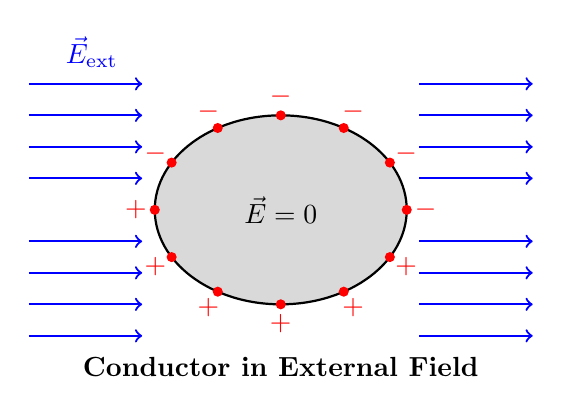
\begin{tikzpicture}[scale=0.8]
    % External field lines
    \foreach \y in {-2,-1.5,-1,-0.5,0.5,1,1.5,2} {
        \draw[->, thick, blue] (-4,\y) -- (-2.2,\y);
        \draw[->, thick, blue] (2.2,\y) -- (4,\y);
    }
    
    % Conductor (ellipse)
    \draw[thick, fill=gray!30] (0,0) ellipse (2 and 1.5);
    \node at (0,0) {$\vec{E} = 0$};
    
    % Surface charges
    \foreach \angle in {0,30,60,90,120,150,180,210,240,270,300,330} {
        \coordinate (pos) at (\angle:2 and 1.5);
        \fill[red] (pos) circle (0.08);
        \ifnum\angle<180
            \node[red] at ([shift=(\angle:0.3)] pos) {$-$};
        \else
            \node[red] at ([shift=(\angle:0.3)] pos) {$+$};
        \fi
    }
    
    \node[blue] at (-3,2.5) {$\vec{E}_{\text{ext}}$};
    \node at (0,-2.5) {\textbf{Conductor in External Field}};
\end{tikzpicture}
\end{center}

\subsubsection{Property 2: Zero Volume Charge Density}
\begin{align*}
    \rho(\vec{r}) = 0 \text{ inside conductor}
\end{align*}

From Gauss's law: $\nabla \cdot \vec{E} = \frac{\rho}{\epsilon_0}$. Since $\vec{E} = 0$ inside, we have $\rho = 0$. This is called \textbf{screening}.

\subsubsection{Property 3: Surface Charge Distribution}
If the conductor has net charge, it must reside entirely on the surface. Since $\vec{E} = 0$ inside, there is no mechanism to support volume charge density.

\subsubsection{Property 4: Equipotential Surface}
\begin{align*}
    V = \text{constant throughout conductor}
\end{align*}

Since $\vec{E} = -\nabla V = 0$, the potential cannot vary within the conductor:
\begin{align*}
    V(b) - V(a) = -\int_a^b \vec{E} \cdot d\vec{l} = 0
\end{align*}

\subsubsection{Property 5: Perpendicular Surface Field}
The electric field just outside the conductor surface is perpendicular to the surface. Any tangential component would cause surface charges to move, violating equilibrium.

\begin{center}
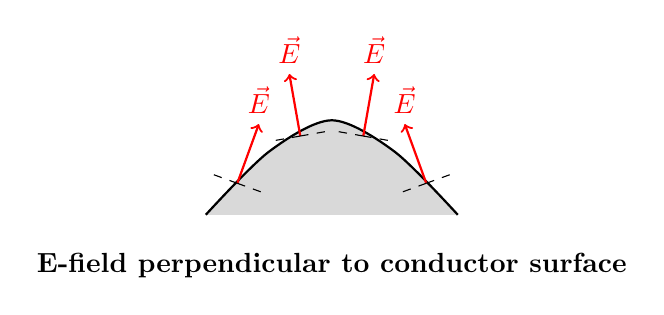
\begin{tikzpicture}[scale=0.8]
    % Conductor surface (curved)
    \draw[thick, fill=gray!30] plot[smooth] coordinates {(-2,-1) (-1,0) (0,0.5) (1,0) (2,-1)};
    
    % Normal vectors at different points
    \foreach \x/\y/\angle in {-1.5/-0.5/70, -0.5/0.25/100, 0.5/0.25/80, 1.5/-0.5/110} {
        \draw[->, thick, red] (\x,\y) -- +(\angle:1) node[above] {$\vec{E}$};
        \draw[dashed] (\x,\y) -- +(\angle+90:0.5);
        \draw[dashed] (\x,\y) -- +(\angle-90:0.5);
    }
    
    \node at (0,-1.8) {\textbf{E-field perpendicular to conductor surface}};
\end{tikzpicture}
\end{center}

\subsubsection{Property 6: Faraday Cage Effect}
A conductor with an internal cavity shields the cavity from external fields. The field inside the cavity is zero regardless of external conditions.

\subsubsection{Property 7: Loss of Spatial Information}
If a charge is placed inside a cavity within a conductor, observers outside the conductor cannot determine the position of the internal charge - only its magnitude affects the external field.

\subsection{Surface Charge and Boundary Conditions}
From our previous boundary condition analysis:
\begin{align*}
    \vec{E}_{\text{above}} - \vec{E}_{\text{below}} = \frac{\sigma}{\epsilon_0}\hat{n}
\end{align*}

For a conductor where $\vec{E}_{\text{below}} = 0$:
\begin{conceptbox}
The electric field just outside a conductor surface is:
\begin{align*}
    \vec{E}_{\text{surface}} = \frac{\sigma}{\epsilon_0}\hat{n}
\end{align*}
where $\sigma$ is the local surface charge density and $\hat{n}$ is the outward normal.
\end{conceptbox}

\subsection{Electrostatic Pressure and Forces}
The electric field exerts a force on the surface charges of a conductor, creating an electrostatic pressure.

\begin{example}[Force per unit area on conductor surface]
Consider the force on a small patch of conductor surface with area $dA$ and charge $dq = \sigma \, dA$.

The field acting on this charge is the average of the field just inside (zero) and just outside ($\sigma/\epsilon_0$):
\begin{align*}
    \vec{E}_{\text{avg}} &= \frac{1}{2}(0 + \frac{\sigma}{\epsilon_0}\hat{n}) = \frac{\sigma}{2\epsilon_0}\hat{n}
\end{align*}

The force per unit area (electrostatic pressure) is:
\begin{align*}
    \vec{P} = \sigma \vec{E}_{\text{avg}} = \frac{\sigma^2}{2\epsilon_0}\hat{n} = \frac{\epsilon_0 E^2}{2}\hat{n}
\end{align*}

This pressure always acts outward, trying to expand the conductor.
\end{example}

\subsection{Introduction to Capacitance}
When we have two conductors at different potentials, we can define capacitance.

\begin{conceptbox}
For two conductors with charges $+Q$ and $-Q$ at potential difference $V$:
\begin{align*}
    C = \frac{Q}{V}
\end{align*}
Units: $[\text{Farad}] = \frac{\text{Coulomb}}{\text{Volt}}$

Capacitance depends only on geometry and material properties, not on $Q$ or $V$.
\end{conceptbox}

The relationship $V \propto Q$ arises because:
\begin{itemize}
    \item Laplace's equation: $\nabla^2 V = 0$ in regions with $\rho = 0$
    \item Boundary conditions: $V = \text{constant}$ on conductor surfaces
    \item Linearity of Laplace's equation ensures $V \propto Q$
\end{itemize}

\begin{example}[Parallel plate capacitor preview]
For two parallel plates with surface charge density $\pm\sigma$:
\begin{align*}
    E &= \frac{\sigma}{\epsilon_0} \\
    V &= Ed = \frac{\sigma d}{\epsilon_0} \\
    Q &= \sigma A \\
    C &= \frac{Q}{V} = \frac{\sigma A}{\sigma d/\epsilon_0} = \frac{\epsilon_0 A}{d}
\end{align*}
\end{example}


%%%%%%%%%%%%%%%%%%%%%%%%%%%%%%%%%%%%%%%%%%%%%%%% New Chapter %%%%%%%%%%%%%%%%%%%%%%%%%%%%%%%%%%%%%%%%%%%%%%%%
\newpage
\section{Lecture 8: Capacitance and Laplace's Equation}
\subsubsection*{September 12, 2025}

\subsection{Recap: Conductor Properties}
From our study of conductors, we established:
\begin{align*}
    V &= V_+ - V_- \quad \text{(potential difference)} \\
    \nabla^2 V &= -\frac{\rho}{\epsilon_0} \quad \text{(Poisson's equation)} \\
    V &\propto Q \quad \text{(linear relationship)}
\end{align*}

\subsection{Capacitance}
\begin{conceptbox}
For two conductors with charges $\pm Q$ at potential difference $V$:
\begin{align*}
    C = \frac{Q}{V}
\end{align*}
Units: $[\text{Farad}] = \frac{\text{Coulomb}}{\text{Volt}}$

Capacitance depends only on geometry and material properties, not on $Q$ or $V$.
\end{conceptbox}

\subsection{Parallel Plate Capacitor}
\begin{example}[Parallel plate capacitor]
Consider two parallel plates with area $A$, separation $d$, carrying charges $\pm Q$.

\begin{center}
\begin{minipage}{0.48\textwidth}
    \centering
    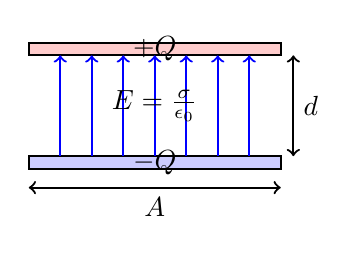
\begin{tikzpicture}[scale=0.8]
        % Bottom plate (-Q)
        \draw[thick, fill=blue!20] (-2,-1) rectangle (2,-0.8);
        \node at (0,-0.9) {$-Q$};
        
        % Top plate (+Q)
        \draw[thick, fill=red!20] (-2,1) rectangle (2,0.8);
        \node at (0,0.9) {$+Q$};
        
        % Electric field lines
        \foreach \x in {-1.5,-1,-0.5,0,0.5,1,1.5} {
            \draw[->, thick, blue] (\x,-0.8) -- (\x,0.8);
        }
        
        % Distance label
        \draw[<->, thick] (2.2,-0.8) -- (2.2,0.8) node[midway, right] {$d$};
        
        % Area label
        \draw[<->, thick] (-2,-1.3) -- (2,-1.3) node[midway, below] {$A$};
        
        % Field magnitude
        \node at (0,0) {$E = \frac{\sigma}{\epsilon_0}$};
    \end{tikzpicture}
\end{minipage}%
\hfill
\begin{minipage}{0.48\textwidth}
    \vspace{0.5em}
    \begin{align*}
        &\text{Using Gauss's law:} \\
        &\oint \vec{E} \cdot d\vec{A} = \frac{Q_{enc}}{\epsilon_0} \\
        &E \cdot A = \frac{\sigma A}{\epsilon_0} \\
        &E = \frac{\sigma}{\epsilon_0} = \frac{Q}{\epsilon_0 A} \\
        &\\
        &\text{Potential difference:} \\
        &V = -\int \vec{E} \cdot d\vec{l} = Ed = \frac{Qd}{\epsilon_0 A} \\
        &\\
        &\text{Capacitance:} \\
        &C = \frac{Q}{V} = \frac{\epsilon_0 A}{d}
    \end{align*}
\end{minipage}
\end{center}
\end{example}

\subsection{Energy Stored in Capacitor}
\begin{conceptbox}
The energy stored in a capacitor can be calculated as:
\begin{align*}
    W &= \int V \, dq = \int_0^Q \frac{q}{C} \, dq = \frac{Q^2}{2C} \\
    &= \frac{1}{2}CV^2 = \frac{1}{2}QV
\end{align*}
\end{conceptbox}

\subsection{General Potential Calculations}
For arbitrary charge configurations, we have two approaches:

\subsubsection{High Symmetry Cases}
When symmetry allows direct integration:
\begin{align*}
    V(\vec{r}) = \frac{1}{4\pi\epsilon_0} \int \frac{\rho(\vec{r}')}{|\vec{r} - \vec{r}'|} \, d\tau'
\end{align*}

\subsubsection{General Cases}
When direct integration is difficult, solve Poisson's equation:
\begin{align*}
    \nabla^2 V(\vec{r}) = -\frac{\rho(\vec{r})}{\epsilon_0}
\end{align*}

\subsection{Example: Hemispherical Shell (Griffiths 2.48)}
\begin{example}[Hemispherical shell potential difference]
An inverted hemispherical bowl of radius $R$ carries uniform surface charge density $\sigma$. Find the potential difference between the "north pole" and the center.

\begin{center}
\begin{minipage}{0.48\textwidth}
    \centering
    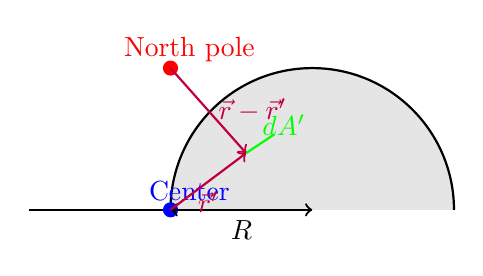
\begin{tikzpicture}[scale=1.2]
        % Hemisphere
        \draw[thick, fill=gray!20] (0,0) arc (180:0:1.5);
        \draw[thick] (-1.5,0) -- (1.5,0);
        
        % North pole
        \fill[red] (0,1.5) circle (0.08);
        \node[red] at (0.2,1.7) {North pole};
        
        % Center
        \fill[blue] (0,0) circle (0.08);
        \node[blue] at (0.2,0.2) {Center};
        
        % Radius
        \draw[<->, thick] (0,0) -- (1.5,0) node[midway, below] {$R$};
        
        % Surface element
        \draw[thick, green] (0.8,0.6) -- (1.1,0.8);
        \node[green] at (1.2,0.9) {$dA'$};
        
        % Distance vectors
        \draw[->, thick, purple] (0,1.5) -- (0.8,0.6) node[midway, right] {$\vec{r} - \vec{r}'$};
        \draw[->, thick, purple] (0,0) -- (0.8,0.6) node[midway, below] {$\vec{r}'$};
    \end{tikzpicture}
\end{minipage}%
\hfill
\begin{minipage}{0.48\textwidth}
    \vspace{0.5em}
    \begin{align*}
        &V(\vec{r}) = \frac{1}{4\pi\epsilon_0} \int \frac{\sigma(\vec{r}')}{|\vec{r} - \vec{r}'|} \, dA' \\
        &\\
        &\text{At center: } |\vec{r} - \vec{r}'| = R \\
        &V_{\text{center}} = \frac{1}{4\pi\epsilon_0} \int \frac{\sigma}{R} \, dA' \\
        &= \frac{\sigma R}{2\epsilon_0} \\
        &\\
        &\text{At north pole: } |\vec{r} - \vec{r}'| = \sqrt{2}R\sqrt{1-\cos\theta} \\
        &V_{\text{pole}} = \frac{\sigma R}{\sqrt{2}\epsilon_0} \\
        &\\
        &\Delta V = V_{\text{pole}} - V_{\text{center}} \\
        &= \frac{\sigma R}{\epsilon_0}\left(\frac{1}{\sqrt{2}} - \frac{1}{2}\right) \\
        &= \frac{\sigma R}{2\epsilon_0}(\sqrt{2} - 1)
    \end{align*}
\end{minipage}
\end{center}
\end{example}

\subsection{Laplace's Equation}
When $\rho = 0$ in a region, we have Laplace's equation:
\begin{conceptbox}
\begin{align*}
    \nabla^2 V = 0
\end{align*}
In Cartesian coordinates:
\begin{align*}
    \frac{\partial^2 V}{\partial x^2} + \frac{\partial^2 V}{\partial y^2} + \frac{\partial^2 V}{\partial z^2} = 0
\end{align*}
\end{conceptbox}

\subsection{Mean Value Theorem}
\begin{theorem}[Mean Value Theorem for Potential]
The potential at the center of a sphere is equal to the average potential over the surface of the sphere, provided there are no charges inside the sphere.
\end{theorem}

\begin{example}[Verification of mean value theorem]
For a point charge $q$ outside a sphere of radius $R$:

\begin{center}
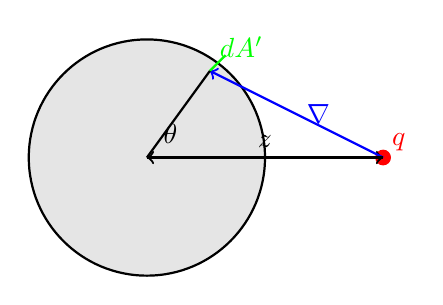
\begin{tikzpicture}[scale=1.0]
    % Sphere
    \draw[thick, fill=gray!20] (0,0) circle (1.5);
    
    % Point charge
    \fill[red] (3,0) circle (0.1);
    \node[red] at (3.2,0.2) {$q$};
    
    % Distance from charge to center
    \draw[<->, thick] (0,0) -- (3,0) node[midway, above] {$z$};
    
    % Distance from charge to surface element
    \draw[->, thick, blue] (3,0) -- (0.8,1.1) node[midway, right] {$\mathcal{r}$};
    
    % Surface element
    \draw[thick, green] (0.8,1.1) -- (1.0,1.3);
    \node[green] at (1.2,1.4) {$dA'$};
    
    % Angle
    \draw[thick] (0,0) -- (0.8,1.1);
    \draw[thick] (0,0) -- (3,0);
    \node at (0.3,0.3) {$\theta$};
\end{tikzpicture}
\end{center}

\begin{align*}
    \mathcal{r} &= \sqrt{z^2 + R^2 - 2zR\cos\theta} \\
    V_{\text{center}} &= \frac{q}{4\pi\epsilon_0 z} \\
    V_{\text{ave}} &= \frac{1}{4\pi R^2} \int \frac{q}{4\pi\epsilon_0 \mathcal{r}} \, dA' \\
    &= \frac{q}{4\pi\epsilon_0 z} = V_{\text{center}}
\end{align*}

This confirms the mean value theorem.
\end{example}

\subsection{Uniqueness Theorem}
\begin{theorem}[Uniqueness of Solutions to Laplace's Equation]
If a function $V$ satisfies Laplace's equation in a region and satisfies the boundary conditions on the surface of that region, then $V$ is unique.
\end{theorem}

This theorem is crucial because it means that if we find any solution to Laplace's equation that satisfies the boundary conditions, we have found the only solution.


%%%%%%%%%%%%%%%%%%%%%%%%%%%%%%%%%%%%%%%%%%%%%%%% New Chapter %%%%%%%%%%%%%%%%%%%%%%%%%%%%%%%%%%%%%%%%%%%%%%%%
\newpage
\section{Lecture 9: The Uniqueness Theorem}
\subsubsection*{September 15, 2025}

\subsection{Recap: Properties of Laplace's Equation}
From our previous study of Laplace's equation for finding potentials $\nabla^2 V = 0$, we established two key properties:

\begin{conceptbox}
Properties of solutions to Laplace's equation:
\begin{enumerate}
    \item \textbf{Mean Value Theorem}: The potential at any point equals the average potential over any sphere centered at that point:
    \begin{align*}
        V(\vec{r}) = \frac{1}{4\pi R^2}\oint V(\vec{r}') \, da'
    \end{align*}
    
    \item \textbf{No Local Extrema}: $V(\vec{r})$ has no local maxima or minima in the interior - extrema occur only at boundaries.
\end{enumerate}
\end{conceptbox}

To solve electrostatic problems, we need both Laplace's equation and appropriate boundary conditions.

\subsection{The Uniqueness Theorem}

\begin{theorem}[Uniqueness Theorem for Electrostatics]
Given boundary conditions on a closed surface, there exists one and only one solution to Laplace's equation (or Poisson's equation) in the volume enclosed by that surface.
\end{theorem}

\subsubsection{Proof for Laplace's Equation}

\textbf{Setup}: Consider a volume $V$ bounded by surface $S$, where we specify $V(\vec{r}) = f(\vec{r})$ on the boundary.

\textbf{Proof by Contradiction}:
Assume two different solutions $V_1$ and $V_2$ exist that both satisfy:
\begin{align*}
    \nabla^2 V_1 &= 0 \quad \text{in } V \\
    \nabla^2 V_2 &= 0 \quad \text{in } V \\
    V_1(\vec{r}) &= V_2(\vec{r}) = f(\vec{r}) \quad \text{on } S
\end{align*}

Define the difference: $V_3 = V_1 - V_2$

Then:
\begin{align*}
    \nabla^2 V_3 &= \nabla^2(V_1 - V_2) = \nabla^2 V_1 - \nabla^2 V_2 = 0 - 0 = 0 \\
    V_3(\vec{r}) &= V_1(\vec{r}) - V_2(\vec{r}) = f(\vec{r}) - f(\vec{r}) = 0 \quad \text{on } S
\end{align*}

Since $V_3$ satisfies Laplace's equation and equals zero on the boundary, and since Laplace's equation has no local extrema in the interior, $V_3$ must be zero everywhere in $V$.

Therefore: $V_3 = 0 \Rightarrow V_1 = V_2$

\subsubsection{Extension to Poisson's Equation}

\begin{theorem}[Uniqueness for Poisson's Equation]
The uniqueness theorem also applies to Poisson's equation: $\nabla^2 V = -\frac{\rho(\vec{r})}{\epsilon_0}$
\end{theorem}

\textbf{Proof}: If $V_1$ and $V_2$ are solutions to Poisson's equation with the same boundary conditions:
\begin{align*}
    \nabla^2 V_3 &= \nabla^2(V_1 - V_2) = -\frac{\rho}{\epsilon_0} - \left(-\frac{\rho}{\epsilon_0}\right) = 0
\end{align*}

The rest follows identically to the Laplace case.

\subsection{Alternative Boundary Conditions}

\begin{conceptbox}
The uniqueness theorem applies to different types of boundary conditions:
\begin{itemize}
    \item \textbf{Dirichlet}: Specify $V(\vec{r})$ on the boundary surface $S$
    \item \textbf{Neumann}: Specify $\frac{\partial V}{\partial n}$ on the boundary surface $S$  
    \item \textbf{Conductor charges}: Specify total charges $Q_i$ on conductor surfaces
\end{itemize}
\end{conceptbox}

\subsubsection{Uniqueness with Conductor Boundary Conditions}

For conductors, we can specify total charges instead of potentials. Consider two electric fields $\vec{E}_1$ and $\vec{E}_2$ that satisfy:
\begin{align*}
    \nabla \cdot \vec{E}_1 &= \nabla \cdot \vec{E}_2 = \frac{\rho(\vec{r})}{\epsilon_0} \\
    \oint_{S_i} \vec{E}_1 \cdot d\vec{a} &= \oint_{S_i} \vec{E}_2 \cdot d\vec{a} = \frac{Q_i}{\epsilon_0} \quad \text{for each conductor } i
\end{align*}

Define $\vec{E}_3 = \vec{E}_1 - \vec{E}_2$. Then:
\begin{align*}
    \nabla \cdot \vec{E}_3 &= 0 \\
    \oint_{S_i} \vec{E}_3 \cdot d\vec{a} &= 0 \quad \text{for each conductor}
\end{align*}

Since conductors are equipotentials, $V_3 = V_1 - V_2$ is constant on each conductor surface.

Using the vector identity and divergence theorem:
\begin{align*}
    \nabla \cdot (V_3 \vec{E}_3) &= V_3(\nabla \cdot \vec{E}_3) + \vec{E}_3 \cdot (\nabla V_3) \\
    &= 0 - \vec{E}_3 \cdot \vec{E}_3 = -E_3^2
\end{align*}

Integrating over the volume:
\begin{align*}
    \int_V \nabla \cdot (V_3 \vec{E}_3) \, d\tau &= \oint_S V_3 \vec{E}_3 \cdot d\vec{a} = -\int_V E_3^2 \, d\tau
\end{align*}

Since $V_3$ is constant on each conductor surface and $\oint_{S_i} \vec{E}_3 \cdot d\vec{a} = 0$, the left side equals zero.

Therefore: $E_3^2 = 0 \Rightarrow \vec{E}_3 = 0 \Rightarrow \vec{E}_1 = \vec{E}_2$

\subsection{Method of Images}

The uniqueness theorem enables powerful solution techniques like the method of images.

\begin{example}[Point charge above grounded conducting plane]
Consider a point charge $q$ at position $(0,0,d)$ above a grounded conducting plane at $z = 0$.

\textbf{Boundary conditions}:
\begin{itemize}
    \item $V(x,y,0) = 0$ (grounded plane)
    \item $V(\vec{r}) \to 0$ as $|\vec{r}| \to \infty$
\end{itemize}

\begin{center}
\begin{minipage}{0.48\textwidth}
    \centering
    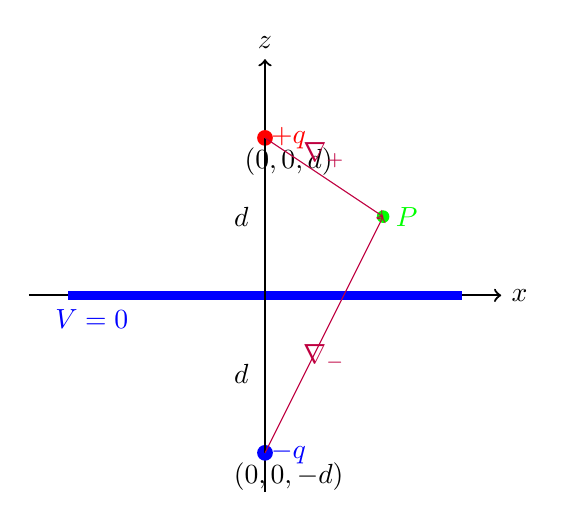
\begin{tikzpicture}[scale=1.0]
        % Coordinate system
        \draw[->, thick] (-3,0) -- (3,0) node[right] {$x$};
        \draw[->, thick] (0,-2.5) -- (0,3) node[above] {$z$};
        
        % Grounded plane
        \draw[thick, blue, line width=3pt] (-2.5,0) -- (2.5,0);
        \node[blue] at (-2.2,-0.3) {$V = 0$};
        
        % Real charge
        \fill[red] (0,2) circle (0.1);
        \node[red] at (0.3,2) {$+q$};
        \node at (0.3,1.7) {$(0,0,d)$};
        
        % Image charge
        \fill[blue] (0,-2) circle (0.1);
        \node[blue] at (0.3,-2) {$-q$};
        \node at (0.3,-2.3) {$(0,0,-d)$};
        
        % Distance markers
        \draw[dashed] (0,0) -- (0,2);
        \draw[dashed] (0,0) -- (0,-2);
        \node at (-0.3,1) {$d$};
        \node at (-0.3,-1) {$d$};
        
        % Field point
        \fill[green] (1.5,1) circle (0.08);
        \node[green] at (1.8,1) {$P$};
        
        % Distance vectors
        \draw[->, purple] (0,2) -- (1.5,1) node[midway, above] {$\mathcal{r}_+$};
        \draw[->, purple] (0,-2) -- (1.5,1) node[midway, below] {$\mathcal{r}_-$};
    \end{tikzpicture}
\end{minipage}%
\hfill
\begin{minipage}{0.48\textwidth}
    \vspace{0.5em}
    \textbf{Solution Strategy}:
    
    Place an image charge $-q$ at $(0,0,-d)$ (outside the region of interest).
    
    \textbf{Potential}:
    \begin{align*}
        V &= \frac{q}{4\pi\epsilon_0 \mathcal{r}_+} - \frac{q}{4\pi\epsilon_0 \mathcal{r}_-}
    \end{align*}
    
    where:
    \begin{align*}
        \mathcal{r}_+ &= \sqrt{x^2+y^2+(z-d)^2} \\
        \mathcal{r}_- &= \sqrt{x^2+y^2+(z+d)^2}
    \end{align*}
    
    \textbf{Verification}:
    \begin{align*}
        V|_{z=0} &= \frac{q}{4\pi\epsilon_0\sqrt{x^2+y^2+d^2}} \\
        &\quad - \frac{q}{4\pi\epsilon_0\sqrt{x^2+y^2+d^2}} = 0 \checkmark
    \end{align*}
\end{minipage}
\end{center}

\textbf{Final Solution}:
\begin{conceptbox}
\begin{align*}
    V(x,y,z) = \frac{q}{4\pi\epsilon_0}\left[\frac{1}{\sqrt{x^2+y^2+(z-d)^2}} - \frac{1}{\sqrt{x^2+y^2+(z+d)^2}}\right]
\end{align*}
\end{conceptbox}

The image charge $-q$ at $(0,0,-d)$ is called the \textbf{image charge}. It can only be placed outside the region where we're solving for the potential. The conductor acts like a mirror, creating the image charge to satisfy boundary conditions.
\end{example}

\subsection{Physical Interpretation}

\begin{center}
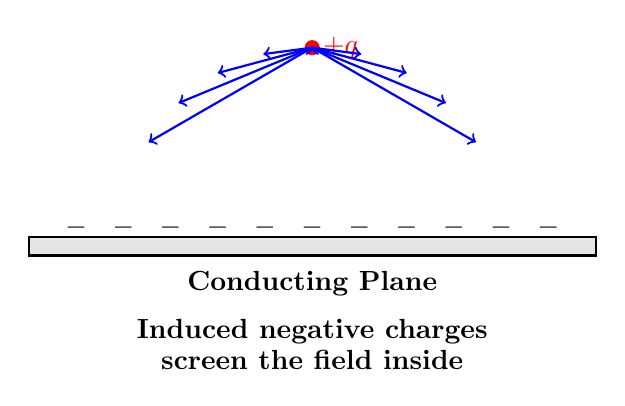
\begin{tikzpicture}[scale=1.2]
    % Draw the conducting plane
    \draw[thick, fill=gray!20] (-3,0) rectangle (3,-0.2);
    \node at (0,-0.5) {\textbf{Conducting Plane}};
    
    % Real charge and field lines above
    \fill[red] (0,2) circle (0.08);
    \node[red] at (0.3,2) {$+q$};
    
    % Draw field lines from charge to plane
    \foreach \angle in {-60,-45,-30,-15,0,15,30,45,60} {
        \draw[->, thick, blue] (0,2) -- ({2*sin(\angle)}, {2*cos(\angle)});
    }
    
    % Surface charges on conductor
    \foreach \x in {-2.5,-2,-1.5,-1,-0.5,0,0.5,1,1.5,2,2.5} {
        \node at (\x,0.1) {$-$};
    }
    
    % Induced charge distribution
    \node at (0,-1) {\textbf{Induced negative charges}};
    \node at (0,-1.3) {\textbf{screen the field inside}};
\end{tikzpicture}
\end{center}

The method of images works because:
\begin{itemize}
    \item The conductor redistributes surface charge to maintain $V = 0$
    \item The image charge mimics this redistribution effect
    \item By uniqueness, this is the only possible solution
\end{itemize}


%%%%%%%%%%%%%%%%%%%%%%%%%%%%%%%%%%%%%%%%%%%%%%%% New Chapter %%%%%%%%%%%%%%%%%%%%%%%%%%%%%%%%%%%%%%%%%%%%%%%%
\newpage
\section{Common Math}
\subsubsection*{}

\subsection{Vector Calculus}

\subsubsection{Vector Operations}
\begin{example}[Vector Dot Product]
The dot product of two vectors:
\begin{align*}
    \vec{A} \cdot \vec{B} &= A_x B_x + A_y B_y + A_z B_z \\
    &= |\vec{A}||\vec{B}|\cos\theta
\end{align*}
\end{example}

\begin{example}[Vector Cross Product]
The cross product in component form:
\begin{align*}
    \vec{A} \times \vec{B} &= \begin{vmatrix}
        \hat{i} & \hat{j} & \hat{k} \\
        A_x & A_y & A_z \\
        B_x & B_y & B_z
    \end{vmatrix} \\
    &= (A_y B_z - A_z B_y)\hat{i} + (A_z B_x - A_x B_z)\hat{j} + (A_x B_y - A_y B_x)\hat{k}
\end{align*}
\end{example}

\subsubsection{Differential Operators}
\begin{example}[Gradient]
The gradient of a scalar function:
\begin{align*}
    \nabla f &= \frac{\partial f}{\partial x}\hat{i} + \frac{\partial f}{\partial y}\hat{j} + \frac{\partial f}{\partial z}\hat{k} \\
    &= \left(\frac{\partial}{\partial x}, \frac{\partial}{\partial y}, \frac{\partial}{\partial z}\right)f
\end{align*}
\end{example}

\begin{example}[Divergence]
The divergence of a vector field:
\begin{align*}
    \nabla \cdot \vec{F} &= \frac{\partial F_x}{\partial x} + \frac{\partial F_y}{\partial y} + \frac{\partial F_z}{\partial z}
\end{align*}
\end{example}

\begin{example}[Curl]
The curl of a vector field:
\begin{align*}
    \nabla \times \vec{F} &= \begin{vmatrix}
        \hat{i} & \hat{j} & \hat{k} \\
        \frac{\partial}{\partial x} & \frac{\partial}{\partial y} & \frac{\partial}{\partial z} \\
        F_x & F_y & F_z
    \end{vmatrix}
\end{align*}
\end{example}

\subsection{Line Integrals and Path Integrals}

\begin{example}[Line Integral of a Vector Field]
Work done by a force along a path:
\begin{align*}
    W &= \int_C \vec{F} \cdot d\vec{r} \\
    &= \int_a^b \vec{F}(\vec{r}(t)) \cdot \frac{d\vec{r}}{dt} dt
\end{align*}
where $\vec{r}(t)$ parametrizes the curve $C$ from $t=a$ to $t=b$.
\end{example}

\begin{example}[Line Integral of a Scalar Field]
Integral of a scalar function along a curve:
\begin{align*}
    \int_C f(x,y,z) \, ds &= \int_a^b f(\vec{r}(t)) \left|\frac{d\vec{r}}{dt}\right| dt
\end{align*}
\end{example}

\begin{example}[Closed Path Integral]
Circulation around a closed loop:
\begin{align*}
    \oint_C \vec{F} \cdot d\vec{r} = \iint_S (\nabla \times \vec{F}) \cdot \hat{n} \, dS
\end{align*}
This is Stokes' theorem.
\end{example}

\subsection{Surface and Volume Integrals}

\begin{example}[Surface Integral]
Flux through a surface:
\begin{align*}
    \Phi &= \iint_S \vec{F} \cdot \hat{n} \, dS \\
    &= \iint_S \vec{F} \cdot \frac{\vec{r}_u \times \vec{r}_v}{|\vec{r}_u \times \vec{r}_v|} |\vec{r}_u \times \vec{r}_v| \, du \, dv
\end{align*}
where $\vec{r}(u,v)$ parametrizes the surface $S$.
\end{example}

\begin{example}[Volume Integral]
Integral over a volume:
\begin{align*}
    \iiint_V f(x,y,z) \, dV &= \iiint_V f(x,y,z) \, dx \, dy \, dz
\end{align*}
\end{example}

\subsection{Differential Equations}

\begin{example}[First-Order Linear ODE]
\begin{align*}
    \frac{dy}{dx} + P(x)y &= Q(x) \\
    \text{Solution: } y &= e^{-\int P(x)dx}\left[\int Q(x)e^{\int P(x)dx}dx + C\right]
\end{align*}
\end{example}

\begin{example}[Second-Order Linear ODE with Constant Coefficients]
\begin{align*}
    \frac{d^2y}{dx^2} + a\frac{dy}{dx} + by &= f(x) \\
    \text{Characteristic equation: } r^2 + ar + b &= 0
\end{align*}
\end{example}

\begin{example}[Wave Equation]
\begin{align*}
    \frac{\partial^2 u}{\partial t^2} &= c^2\nabla^2 u \\
    \frac{\partial^2 u}{\partial t^2} &= c^2\left(\frac{\partial^2 u}{\partial x^2} + \frac{\partial^2 u}{\partial y^2} + \frac{\partial^2 u}{\partial z^2}\right)
\end{align*}
\end{example}

\subsection{Complex Numbers and Phasors}

\begin{example}[Complex Exponential]
Euler's formula and complex representation:
\begin{align*}
    e^{i\theta} &= \cos\theta + i\sin\theta \\
    z &= re^{i\theta} = r(\cos\theta + i\sin\theta)
\end{align*}
\end{example}

\begin{example}[Phasor Notation]
AC voltage representation:
\begin{align*}
    V(t) &= V_0\cos(\omega t + \phi) \\
    \tilde{V} &= V_0e^{i\phi} \quad \text{(phasor)}
\end{align*}
\end{example}

\subsection{Series and Summations}

\begin{example}[Taylor Series]
\begin{align*}
    f(x) &= f(a) + f'(a)(x-a) + \frac{f''(a)}{2!}(x-a)^2 + \cdots \\
    &= \sum_{n=0}^{\infty} \frac{f^{(n)}(a)}{n!}(x-a)^n
\end{align*}
\end{example}

\begin{example}[Fourier Series]
\begin{align*}
    f(x) &= \frac{a_0}{2} + \sum_{n=1}^{\infty} \left[a_n\cos\left(\frac{n\pi x}{L}\right) + b_n\sin\left(\frac{n\pi x}{L}\right)\right] \\
    a_n &= \frac{1}{L}\int_{-L}^L f(x)\cos\left(\frac{n\pi x}{L}\right)dx \\
    b_n &= \frac{1}{L}\int_{-L}^L f(x)\sin\left(\frac{n\pi x}{L}\right)dx
\end{align*}
\end{example}

\subsection{Coordinate Systems}

\begin{example}[Spherical Coordinates]
\begin{align*}
    x &= r\sin\theta\cos\phi \\
    y &= r\sin\theta\sin\phi \\
    z &= r\cos\theta \\
    dV &= r^2\sin\theta \, dr \, d\theta \, d\phi
\end{align*}
\end{example}

\begin{example}[Cylindrical Coordinates]
\begin{align*}
    x &= \rho\cos\phi \\
    y &= \rho\sin\phi \\
    z &= z \\
    dV &= \rho \, d\rho \, d\phi \, dz
\end{align*}
\end{example}

\subsection{Special Functions}

\begin{example}[Dirac Delta Function]
\begin{align*}
    \delta(x) &= \begin{cases}
        \infty & \text{if } x = 0 \\
        0 & \text{if } x \neq 0
    \end{cases} \\
    \int_{-\infty}^{\infty} \delta(x) \, dx &= 1 \\
    \int_{-\infty}^{\infty} f(x)\delta(x-a) \, dx &= f(a)
\end{align*}
\end{example}

\begin{example}[Heaviside Step Function]
\begin{align*}
    H(x) &= \begin{cases}
        1 & \text{if } x > 0 \\
        0 & \text{if } x < 0
    \end{cases} \\
    \frac{d}{dx}H(x) &= \delta(x)
\end{align*}
\end{example}

\subsection{Matrix Operations}

\begin{example}[Eigenvalue Problem]
\begin{align*}
    A\vec{v} &= \lambda\vec{v} \\
    \det(A - \lambda I) &= 0
\end{align*}
\end{example}

\begin{example}[Matrix Exponential]
\begin{align*}
    e^A &= \sum_{n=0}^{\infty} \frac{A^n}{n!} \\
    &= I + A + \frac{A^2}{2!} + \frac{A^3}{3!} + \cdots
\end{align*}
\end{example}

\subsection{Statistical Physics}

\begin{example}[Boltzmann Distribution]
\begin{align*}
    P(E) &= \frac{1}{Z}e^{-\beta E} \\
    Z &= \sum_i e^{-\beta E_i} \quad \text{(partition function)} \\
    \beta &= \frac{1}{k_B T}
\end{align*}
\end{example}

\begin{example}[Maxwell-Boltzmann Distribution]
\begin{align*}
    f(v) &= 4\pi v^2\left(\frac{m}{2\pi k_B T}\right)^{3/2}e^{-mv^2/(2k_B T)}
\end{align*}
\end{example}

\end{document}